In order to test the possibilities of WFS applied to cancellation of noise in the anechoic chamber, an appropriate software tool is required. The development of that tool, called WFSTool and written in Matlab, has been the result of this thesis.

The main capability of WFSTool is to play a sinusoidal signal of a desired frequency $f$ through one or more loudspeakers that will act as noise sources and, at the same time, play through each loudspeaker of the WFS array a sinusoidal signal of the same frequency $f$ but with different amplitudes and phases, so the interference of the acoustic field generated by the noise sources and the WFS array interfere destructively, in the ideal case. The acoustic field will be recorded by microphones located in the area of interest, so then can be analysed. To understand how the program works, we are going to cover the different blocks that are executed during the generation and reproduction of the signals.

\begin{figure}
	\centering
	\def\svgwidth{1\columnwidth}
	\graphicspath{{Img/}}
	\input{Img/pruebaPDFLatex.pdf_tex}
	\caption{WFSTool scheme}
	\label{figprueba}
\end{figure}

\begin{figure}
	\centering
	\def\svgwidth{1\columnwidth}
	\graphicspath{{Img/}}
	\input{Img/WFSToolSchemeReport.pdf_tex}
	\caption{WFSTool scheme}
	\label{figWFSToolScheme}
\end{figure}

\subsection{Setup of the scenario}
The starting point is the set up of relevant parameters in the mathematical modelling of the scenario, as described in \autoref{TheoreticalModelLabel}.

We need to set, at first, the properties of the WFS array. This is, the position (3D coordinates) all the loudspeakers and their radiation patterns (function with relative position as input argument). In the case of the anechoic chamber we use, there are 96 loudspeakers distributed as an polygon as it is showed in \autoref{WFSdistribution}. For simplification purposes, we have assumed that they are isotropic sources, but the software can work with any radiation pattern.

Once we have modelled the WFS array, we need to set the properties of the noise sources. They will also have a position, orientation and radiation pattern. But also the complex coefficient of the transmitted signal. The program allows to specify if the source is virtual, real, or both. If a noise source is declared as virtual, it means that it will be considered in the WFS calculation to generate a field that will interfere destructively. If a noise source is real, it means that the signal will actually be reproduced by a loudspeaker. In that case, we need to specify the channel that will be used for that purpose. Of course, the normal configuration in our experiment is that noise sources are both real and virtual.

The same must be done with the microphones, that will also have a position, orientation and radiation pattern. It is also needed to specify the channel number of the recording device to which each microphone is connected.
 
\subsection{WFS calculation}
\label{WFScalculation}

Now the scenario is theoretically defined. The next step is the application of the WFS calculations in order to generate the appropriate complex coefficients that will create a field for the noise cancellation. Actually, it consists in generating the field that an hypothetical noise source (virtual noise source) equal to the real one but with opposite sign would produce. This way, both fields would cancel each other (the sum will be $0$). It takes in account the position of the noise source and loudspeakers, and the orientation of the latter. The information about the radiation patterns set by the user are not used. However, in future modifications of the software a more sophisticated WFS calculation that uses more information could be used. The calculations are particularized for the loudspeaker array in the anechoic chamber. These calculations were provided by the professors and require much professional knowledge in the physic area, which is not an important section of the project.

The original noise signal will be scaled by an attenuation coefficient and delayed a certain amount of time. The attenuation is calculated by determining the distance between the source and the loudspeaker $d$ and the angle $\alpha$ between the vector that goes from the source to the loudspeaker and the loudspeaker's broadside direction.
\begin{equation}
\begin{aligned}
a &= A\frac{\cos\alpha}{\sqrt{d}} \\
A &= \sqrt{\frac{r_0}{r_0 + d}}\\
r_0 &= \frac{1.44}{2} + 1.44 \cos\left( \frac{\pi}{4} \right)
\end{aligned}
\label{WFScalcEqObsolete}
\end{equation}

The delay time is actually the time it takes for the sound transmitted by the noise source to reach the loudspeaker. It is related to the distance $d$ and the propagation velocity of acoustic waves in air $c = 343 (m/s)$.
\begin{equation}
\tau = \frac{d}{c} \label{WFScalcEqDelayObsolete}
\end{equation}

Finally, there is a condition that must be met in order to activate a loudspeaker. If the angle $\alpha$ is smaller than $90^\circ$, then the loudspeaker is active. In other case, is not enabled.

\subsection{Reproduction and Recording}
After WFS, the system is ready to be tested. We have defined a signal for every loudspeaker, and we know theoretically their position, orientation and radiation pattern. The next step is the reproduction and recording.

This step is delicate because the software must use the audio driver and several parameters must be configured. The class ReproductorRecorder has been developed in Matlab in order to manage all reproduction issues and make the communication with audio drivers transparent to the user.

Although the class ReproductorRecorder is able to play many types of signals on multiple devices simultaneously, apply real-time processing, and other features, the use that is given in the program is relatively simple. In the program we work with sinusoidal pulses. Each pulse is defined by its duration, frequency and complex coefficient (amplitude and phase).

Then, a signal is perfectly defined by a 3D array \variable{pulseCoefMat}, a 2D array \variable{pulseLimits}, and 2 vectors (\variable{channels} and \variable{frequencies}). The size of the matrix is ($numPulses$, $numChannels$, $numFrequencies$), and the ($p$, $ch$, $f$)-th element is the complex coefficient of the $p$-th pulse, reproduced by the \variable{channels[ch]} channel in the playing device, with frequency \variable{frequencies[f]}. The starting end ending time of the pulses are \variable{pulseLimits[p, 1]} and \variable{pulseLimits[p, 2]} respectively.

A way of expressing it is that the signal of the $j$-th channel is:
\begin{equation}
x_{ch}(t) = \sum_{f = 1}^{F} \sum_{p = 1}^{P} W\left(\frac{t - \tau_p}{T_p}\right)
\Re \left\{ \myMatrix{C}_{(p,ch,f)} e^{j 2 \pi \vec{F}_f t} \right\}
\end{equation}

\begin{description}
	\item[$\myMatrix{C}$] Pulse coefficient matrix \variable{pulseCoefMat}
	\item[$\vec{F}$] Frequency vector \variable{frequencies}
	\item[$W(t)$] Window function
	\item[$numF$] Number of frequencies $numFrequencies$
	\item[$numP$] Number of pulses $numPulses$
	\item[$\tau_p$] Delay of the midpoint $p$-th pulse: $\frac{\text{\variable{pulseLimits[p, 1] + pulseLimits[p, 2]}}}{2}$
	\item[$T_p$] Duration of the $p$-th pulse: $\text{\variable{pulseLimits[p, 2] - pulseLimits[p, 1]}}$
\end{description}

The window $W$ can be a rectangular function as defined in \autoref{rectFunc}. However, other functions with a different spectrum can be used in order facilitate the detection. During the experiments we have used a modification of the Hanning window to reduce the magnitude of side lobes (\autoref{HanningSpectrumComparison}).
\begin{equation}
\Pi(t) = \left\{ \begin{array}{lcc}
0 &   if  & |t| > 1/2 \\
1 &  if & |t| \leq 1/2 \\
\end{array} \right.
\label{rectFunc}
\end{equation}


For example, the next configuration
\begin{gather*}
\text{\variable{pulseCoefMat[:, :, 1]}} = 
\begin{bmatrix}
	1 & -1 \\
	0 & 0 \\
	0 & 0 \\
	i & 1 \\
\end{bmatrix}
\quad
\text{\variable{pulseCoefMat[:, :, 2]}} = 
\begin{bmatrix}
	0 & 0 \\
	1 & 0 \\
	0 & i \\
	0 & 0 \\
\end{bmatrix}\\
\text{\variable{pulseLimits}} =
\begin{bmatrix}
	1 & 2 \\
	3 & 4 \\
	5 & 7 \\
	9 & 10 \\
\end{bmatrix}
\quad
\text{\variable{channels}} =
\begin{bmatrix}
	2 \\
	1 \\
\end{bmatrix}
\quad
\text{\variable{frequencies}} =
\begin{bmatrix}
	4 \\
	8 \\
\end{bmatrix}
\end{gather*}

gives as a result the signal in the \reffig{examplePulseSignal}.

\begin{figure}[h]
	\centering
	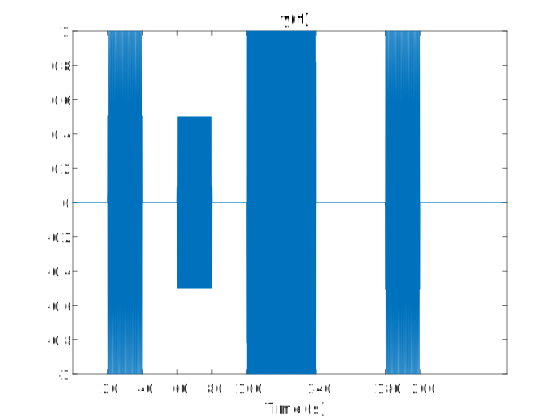
\includegraphics[width=0.4\textwidth]{Img/pulseSignal.eps}
	\caption[Pulse Signal]{Example of pulse signal}
	\label{examplePulseSignal}
\end{figure}

Once the signal has been defined and constructed, it is played and recorded by the class \class{ReproductorRecorder}. The recorded signal is of course different from the transmitted one. It has been modified by the response of loudspeakers and microphones, the noise, the directivity, position of objects, etc. However, we must detect the pulses in order to calculate how the amplitude and phase has been modified. So, how is the detection performed?

\subsection{Detection of pulses}
We take advantage of the fact that we know what the transmitted signal is. So what we are interested in is not detecting the frequency, which we already know, but the complex coefficients of each pulse.

The first step is then to calculate the IQ signal, this is, the low frequency signal that modulates the carrier, whose frequency we know. The relation of the IQ signal and the original one is:
\begin{equation}
x(t) = \Re\{ e^{j 2 \pi f t} x_{IQ}(t) \} = |x_{IQ}(t)| \cos(2 \pi f t + \phi(t))
\label{IQcondition}
\end{equation}
It can be done by applying a band-pass filter around the desired frequency and down-converting the resulting signal (\reffig{detectionScheme}).
\begin{figure}[h]
	\centering
	\includegraphics[width=0.9\textwidth]{Img/detectionScheme.pdf}
	\caption[Detection Scheme]{Scheme of the detection}
	\label{detectionScheme}
\end{figure}

Now that we have the modulating signal $x_{IQ}(t)$, we need to detect where the pulses are. Their amplitude and phase can change, and they can be distorted by noise and non-linear effects, but the duration and delay between them is going to be approximately the same. Hence, we can generate a mask that is set to one when there is a pulse in the original signal and to zero otherwise, cross-correlate it by $x_{IQ}(t)$, and find the lag that returns the maximum value of correlation. To find the complex coefficients of pulses (amplitude and phase), we just perform the mean of each pulse.

\subsection{Calibration}
However, there is a problem that must be solved. Calibration...
